\documentclass[small,algo]{dushClass} %,nocolor,twoside


\title{TP -- Initialisation aux Frameworks}
\subtitle{Hibernate}

\begin{document}

\section{Installation du poste de travail}

\subsection{Les outils}
\begin{description}
\item[Eclipse] : utiliser la version \emph{SpringSource Tools Suite} qui contient déjà tous les plugins nécessaires.
\item[Maven] : outils de gestion de dépendance, de compilation
\item[HSQL DB] : base de données ne nécessitant pas d'installation
\item[Cygwin] : (facultatif) console type Linux (inutile sous la VM)
\item[Git] : (facultatif) gestionnaire de version (type svn)
\end{description}

\subsection{Configuration du poste}

\subsubsection{Système minimum}

\begin{enumerate}
\item Installer \emph{SpringSource Tools Suite} (Eclipse) : il contient une installation de \emph{Maven}
\item Configurer \emph{Maven} pour qu'il puisse accéder à internet (cf annexes \vpageref{mvn-settings})
\item Copier les sources. Il est possible d'utiliser la commande git : \texttt{git clone $<$emplacement des sources$>$ }
\item Importer sous Eclipse (Fichier $\rightarrow$ Import, puis, Maven $\rightarrow$ Existing project)
\end{enumerate}

\subsubsection{Facultatif}

\begin{enumerate}
\item Installer \emph{Cygwin} avec le module Git
\item Modifier le fichier \texttt{.bashrc} pour qu'il puisse accéder à internet et avoir les binaires de Maven dans le path.*
\lstset{language=BASH}
\begin{lstlisting}
# Maven
export PATH=$PATH:/cygdrive/d/Utilitaires/springsource/apache-maven-3.0.4/bin
export JAVA_HOME="C:\Program Files\Java\jdk1.7.0"
# Donne acces a internet a GIT
export http_proxy=http://yr990200:<password>@yrproxy01:8080
export https_proxy=http://yr990200:<password>@yrproxy01:8080
\end{lstlisting}
\end{enumerate}
\lstset{language=JAVA}



%%%%%%%%%%%%%%%%%%%%%%%%%%%%%%%%%%%%%%%%
%% Présentation
\section{Présentation de l'environnement}

\subsection{Sujet du TP}

Nous nous proposons de réaliser l'application de gestion des livres d'une librairie. Les fonctionnalités et les composants évolueront au fil des TP, et des frameworks utilisés.\\

Dans cette première étape, \textbf{Hibernate} est utilisé pour interagir avec la base de données. Le modèle simplifié est présenté figure \ref{model-base} \vpageref{model-base}.

\begin{figure}[ht]
	\center
	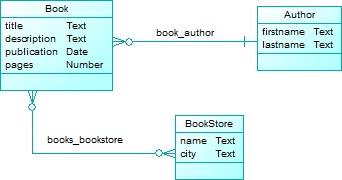
\includegraphics{images/simple_model.png}
	\caption{Modèle simplifié}\label{model-base}
\end{figure}


\subsection{Structure du projet}

\subsubsection{Maven}

Le fichier \emph{Maven} \texttt{pom.xml} est déjà créé.\\

Il décrit le projet comme une application Java se présentant sous forme de \emph{jar} et ayant comme dépendances, entre autre :
\begin{itemize}
\item Hibernate et le drivers HSQL (version 2.x)
\item Logging (SQL4J via LOG4J)
\item Outils liés à JUNIT (junit, festassert, mockito)
\end{itemize}

\subsubsection{Arborescence}

Le projet se présente sous forme de la convention \emph{Maven} :
\begin{itemize}
\item \texttt{src/main/java} : sources JAVA de l'application
\item \texttt{src/main/resources} : ressources et fichiers de configuration
\item \texttt{src/test/java} : sources des tests unitaires
\item \texttt{src/test/resources} : ressources pour les tests unitaires
\end{itemize}

\subsubsection{Base de données}

La base de données conseillée est une base de données \emph{HSQL}. N'importe quelle autre base de données locale pourrait être utilisée.\\

Pour démarrer la BDD, double cliquez sur \texttt{runServer.bat}. Pour visualiser ce qu'il se trouve dedans, double cliquez sur \emph{runManagerSwing.bat} et indiquez l'URL : \texttt{jdbc:hsqldb:hsql://localhost/} comme montré sur la figure \ref{hsqldb-connect} \vpageref{hsqldb-connect}.\\

Hibernate s'occupera de supprimer et créer le schéma à chaque exécution.

\begin{figure}[ht]\label{hsqldb-connect}
	\center
	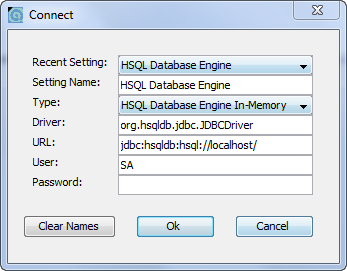
\includegraphics{images/hsqldb_connect.png}
	\caption{Connexion à la base de données HSQL locale}
\end{figure}


\subsection{Configuration des frameworks}

L'objectif étant d'apprendre l'utilisation des frameworks, ils sont pré-configurés.

\subsubsection{Hibernate}

Hibernate est configuré dans le fichier \texttt{src/main/resources/hibernate.cfg.xml}. Y sont définis :
\begin{itemize}
\item les paramètres de la base de données (url, driver, dialecte SQL)
\item les entités (classes persistantes)
\item le schéma de la base sera supprimé et recréé à chaque exécution du programme\\
\end{itemize}

Ce qui correspond aux paramètres de la \texttt{SessionFactory}. Pour accéder à cette dernière, il faut passer par la classe \texttt{HibernateUtils}.

\subsubsection{SLF4J}
Le loggeur est configuré pour afficher l'ensemble des requêtes SQL exécutées par Hibernate. Le fichier de configuration est \texttt{src/main/resources/log4j.properties}.

\subsection{Code}

\subsubsection{Le modèle}

Les première classes sont déjà écrites pour gagner du temps. Elles sont présentes dans le package \texttt{net.yvesrocher.training.frameworks.dto.model}.\\

Pour rappel, DTO correspond à "Data Transfer Object", ou en français \emph{objet de transfert de données}. Il représente les données qui seront persistantes\footnote{persistantes : conservées même en cas d'arrêt de l'application}. Il ne contient \textbf{que} des données (et leurs accesseurs), pas de méthode fonctionnelle !

\subsubsection{Classe \emph{main}}

Afin d'aller droit au but, ce TP se fera directement dans la méthode \texttt{main} (point d'entrée de l'application) et sera lancé via Eclipse. De plus, la classe contient des méthodes pour générer un petit jeu de test.


\section{Travaux pratiques}

Après avoir pris connaissance des différents constituants du projet et de sa structure, passons au développement de l'\emph{interaction avec la base de données}.

\subsection{Mon premier mapping de classe}

Dans un premier temps, nous ne nous intéresseront qu'à la classe \texttt{Book}.

\subsubsection{Sauvegarde d'une entité simple (sans relation) : \texttt{Book}}

\begin{enumerate}
\item mappez la classe \texttt{Book} afin de la rendre \emph{persistante}.
\item testez la sauvegarde d'un nouveau livre
\item regardez via l'interface d'HSQL ce qu'il s'est produit :
\begin{itemize}
\item création du schéma et de la structure de la table (nom et type des colonnes)
\item l'insertion d'un enregistrement (le livre)
\end{itemize}
\end{enumerate}

\subsubsection{Lister les livres présents en base}

Sauvegardez plusieurs livres et cherchez à :
\begin{itemize}
\item les lister (tous)
\item en charger qu'un à partir de son ID : l'afficher, puis le modifier\par
Est-ce nécessaire d'appeler la méthode \texttt{saveOrUpdate} après l'avoir modifier ? Est-ce possible de créer un autre objet \texttt{Book}, de lui donner la même ID, et d'appeler la méthode de sauvegarde ?
\item rechercher les livres parus avant 1980, ou entre 1950 et 2000
\item en supprimer un\\
\end{itemize}

Attention : le schéma est dropé à chaque exécution de la méthode \texttt{main}. Il faut donc que les données soient insérés au début de la méthode main. Ce comportement est défini dans la configuration \emph{Hibernate}.
\subsubsection{Adapter la structure des tables}

\begin{enumerate}
\item modifier le nom de certaines colonnes, regarder le résultat dans la base de données
\item modifier le nom de la table
\end{enumerate}

\subsection{Association avec les classes \texttt{Author} et \texttt{BookStore}}

Dans cette partie, il est conseillée de d'abord travailler sur le mapping d'\texttt{Author} et seulement après passer à \texttt{BookStore}.\\

\begin{enumerate}
\item Déclarer comme persistantes les classes \texttt{Author} et \texttt{BookStore}
\item Dé-commentez les attributs dans la classe \texttt{Book} et configurer les associations
\item Que se passe-t-il quand on sauvegarde un \texttt{Book} qui est lié à un auteur ? Inversement ?
\item Modifier un livre ou un auteur, en le chargeant via son ID, puis en créant une nouvelle instance avec la même ID.
\end{enumerate}

\subsection{Quelques idées de requêtes de recherche}
\begin{itemize}
\item Recherche de livres à partir de l'ID de l'auteur
\item Recherche de livres à partir d'un nom d'auteur
\item Recherche des auteurs dont des ouvrages sont présents dans une ville (on connait les villes des librairies).
\item Recherche des auteurs qui ont écrit au moins 2 livres
\item Recherche des livres présents dans au moins 2 libraires
\item Recherche des auteurs dont au moins 2 livres sont présents dans un librairie données.
\end{itemize}


\section{Pour aller plus loin ...}
Pour aller plus loin, mapper le modèle présenté sur la figure \ref{model-real} \vpageref{model-real}.\\

On intègre l'idée de \texttt{BookCopy} : un exemplaire d'un livre.\\

\begin{figure}[ht]
	\center
	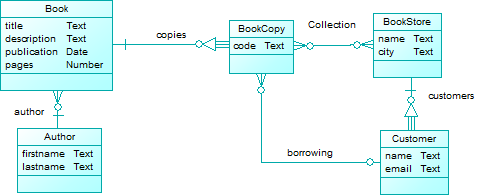
\includegraphics{images/model_real.png}
	\caption{Modèle complet}\label{model-real}
\end{figure}

Exemple de recherche : 
\begin{itemize}
\item lister les références d'un livre présent dans une ville.
\item liste les références encore disponibles (au moins un exemplaire n'a pas été emprunté)
\end{itemize}

\section{Pour aller encore plus loin}

Gestion de l'héritage : introduction de la classe \texttt{Person} dont héritent \texttt{Customer} et \texttt{Author}. Voir figure \ref{model-inheritance} \vpageref{model-inheritance}.\\


\begin{figure}[ht]
	\center
	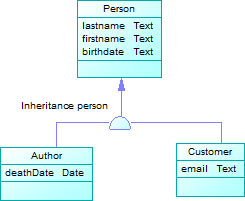
\includegraphics{images/model_inheritance.png}
	\caption{Modèle avec héritage}\label{model-inheritance}
\end{figure}

\begin{enumerate}
\item Tester les différentes stratégie d'héritage (une seule table, 2 tables -- une par classe, 3 tables -- mutualisation des paramètres communs dans une table).
\item Pour chaque stratégie, essayer quelques requêtes : recherche d'auteurs ou de clients, puis recherche de personne en générale.
\item Un héritage au sens base de données est-il une si bonne idée dans ce cas ? Trouver une solution sans héritage en base à proprement parlé.
\end{enumerate}

\cleardoublepage
\section{Annexes}
\lstset{language=XML}

\subsection{Configuration du poste}

\subsubsection{Configuration de \emph{Maven} : \texttt{.m2/settings.xml}}\label{mvn-settings}

\begin{figure}[H]\label{mvn-settings-sts}
	\center
	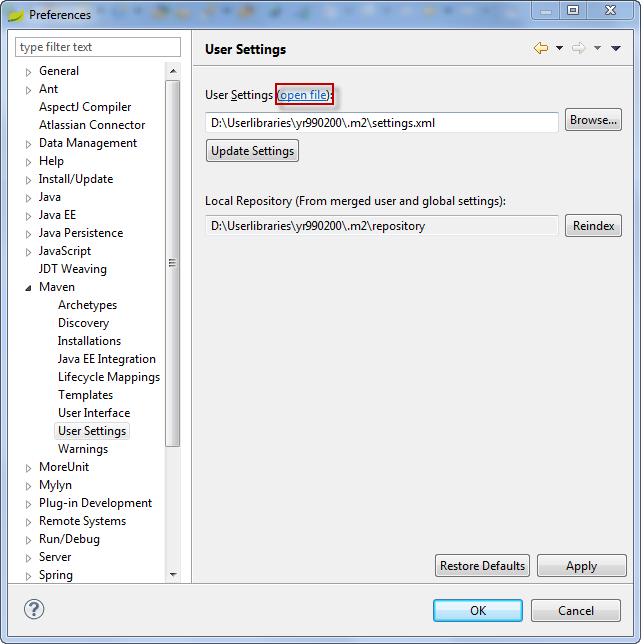
\includegraphics{images/mvn_config.png}
	\caption{Éditer le fichier de configuration via éclipse}
\end{figure}

\begin{lstlisting}
<settings>
  <proxies>  
    <proxy>
      <active>true</active>
      <protocol>http</protocol>
      <host>yrproxy01</host>
      <port>8080</port>
      <username>user</username>
      <password>password</password>
    </proxy>
    <proxy>
      <active>true</active>
      <protocol>https</protocol>
      <host>yrproxy01</host>
      <port>8080</port>
      <username>user</username>
      <password>password</password>
    </proxy>    
  </proxies>  
</settings>

\end{lstlisting}


\end{document}
